\section{Diversification and Portfolios}
\label{sec:diversification_and_portfolios}

By now we have an understanding of how to estimate the expected return of an asset using the Capital Asset Pricing Model (CAPM), and 
how risk and return should have a proportional relationship. In this section we introduce the concept of diversification, and how it can be used to
construct efficient portfolios.

\subsection{The Simple Math of Diversification}
% Explain the expected reutrn math of a portfolio
% Explain the risk math of a portfolio
% ... diversification gets rid of idiosyncratic risk.

\begin{equation}
    \label{eq:portfolio_expected_return}
      E[R_p] = \sum_{i=1}^n w_i E[R_i]
\end{equation}

Where:
\begin{itemize}
    \item $E[R_p]$ is the expected return of the portfolio
    \item $w_i$ is the weight of asset $i$ in the portfolio
    \item $E[R_i]$ is the expected return of asset $i$
    \item $n$ is the number of assets in the portfolio
    \item $w_i$ is the weight of asset $i$ in the portfolio
    \item $E[R_i]$ is the expected return of asset $i$
\end{itemize}

The expected return of a portfolio is simply the weighted average of the expected returns of the assets in the portfolio.

\begin{equation}
    \label{eq:portfolio_risk}
    \sigma_p^2 = \sum_{i=1}^n w_i^2 \sigma_i^2 + \sum_{i=1}^n \sum_{j=1}^n w_i w_j \sigma_{ij}
\end{equation}
Where:
\begin{itemize}
    \item $\sigma_p^2$ is the variance of the portfolio
    \item $w_i$ is the weight of asset $i$ in the portfolio
    \item $\sigma_i^2$ is the variance of asset $i$
    \item $\sigma_{ij}$ is the covariance between assets $i$ and $j$
    \item $n$ is the number of assets in the portfolio
    \item $w_i$ is the weight of asset $i$ in the portfolio
 \end{itemize}
The variance of a portfolio is the weighted average of the variances of the assets in the portfolio, plus the covariance between the assets.
Since we square the weights, and they are between 0 and 1, the variance of the portfolio is always less than or equal to the weighted average of the variances of the assets in the portfolio.
This means that as we add more assets to the portfolio, the variance of the portfolio will decrease, and the expected return will increase.
This is the essence of diversification, and it is the reason why we can construct portfolios that have a higher expected return for a given level of risk.

\subsection{Efficient Portfolios}
% For a given level of risk, there is an optimal portfolio, the markowitz MVO portfolio.
The Markowitz Mean-Variance Optimization (MVO) portfolio is the optimal portfolio for a given level of risk. 
It is the portfolio that has the highest expected return for a given level of risk, or the lowest risk for a given level of expected return.
This is done by solving the following optimization problem:
\begin{equation}
    \label{eq:mvo_optimization}
    \begin{aligned}
        & \text{maximize} && E[R_p] \\
        & \text{subject to} && \sigma_p^2 = \sigma^2 \\
        & && w_i \geq 0, \forall i
    \end{aligned}
\end{equation}
Where:
\begin{itemize}
    \item $E[R_p]$ is the expected return of the portfolio
    \item $\sigma_p^2$ is the variance of the portfolio
    \item $\sigma^2$ is the target variance
    \item $w_i$ is the weight of asset $i$ in the portfolio
    \item $n$ is the number of assets in the portfolio
    \item $w_i$ is the weight of asset $i$ in the portfolio
\end{itemize}

Lets say that we can't short-sell, or take leverage, therefore we have the constraint that $1 \geq w_i \geq 0, \forall i$.

This has a closed form solution:
\begin{equation}
    \label{eq:mvo_closed_form}
    w_i = \frac{E[R_i] - R_f}{\sigma_i^2} \sum_{j=1}^n \frac{E[R_j] - R_f}{\sigma_j^2}
\end{equation}
Where:
\begin{itemize}
    \item $E[R_i]$ is the expected return of asset $i$
    \item $R_f$ is the risk-free rate
    \item $\sigma_i^2$ is the variance of asset $i$
    \item $w_i$ is the weight of asset $i$ in the portfolio
    \item $n$ is the number of assets in the portfolio
\end{itemize}

The weights of the assets in the portfolio are given by the difference between the expected return of the asset and the risk-free rate, divided by the variance of the asset.
This means that the higher the expected return of the asset, the higher the weight in the portfolio, and the lower the variance of the asset, the higher the weight in the portfolio.

\subsection{The Efficient Frontier}
% We now show the efficiennt frontier, and how to ocnstruct it.
The efficient fron tier is just the set of all efficient portfolios.
We can see this visually in figure \ref{fig:efficient_frontier}, where we plot the expected return of every efficient portfolio at every level of risk.

\begin{figure}
    \centering
    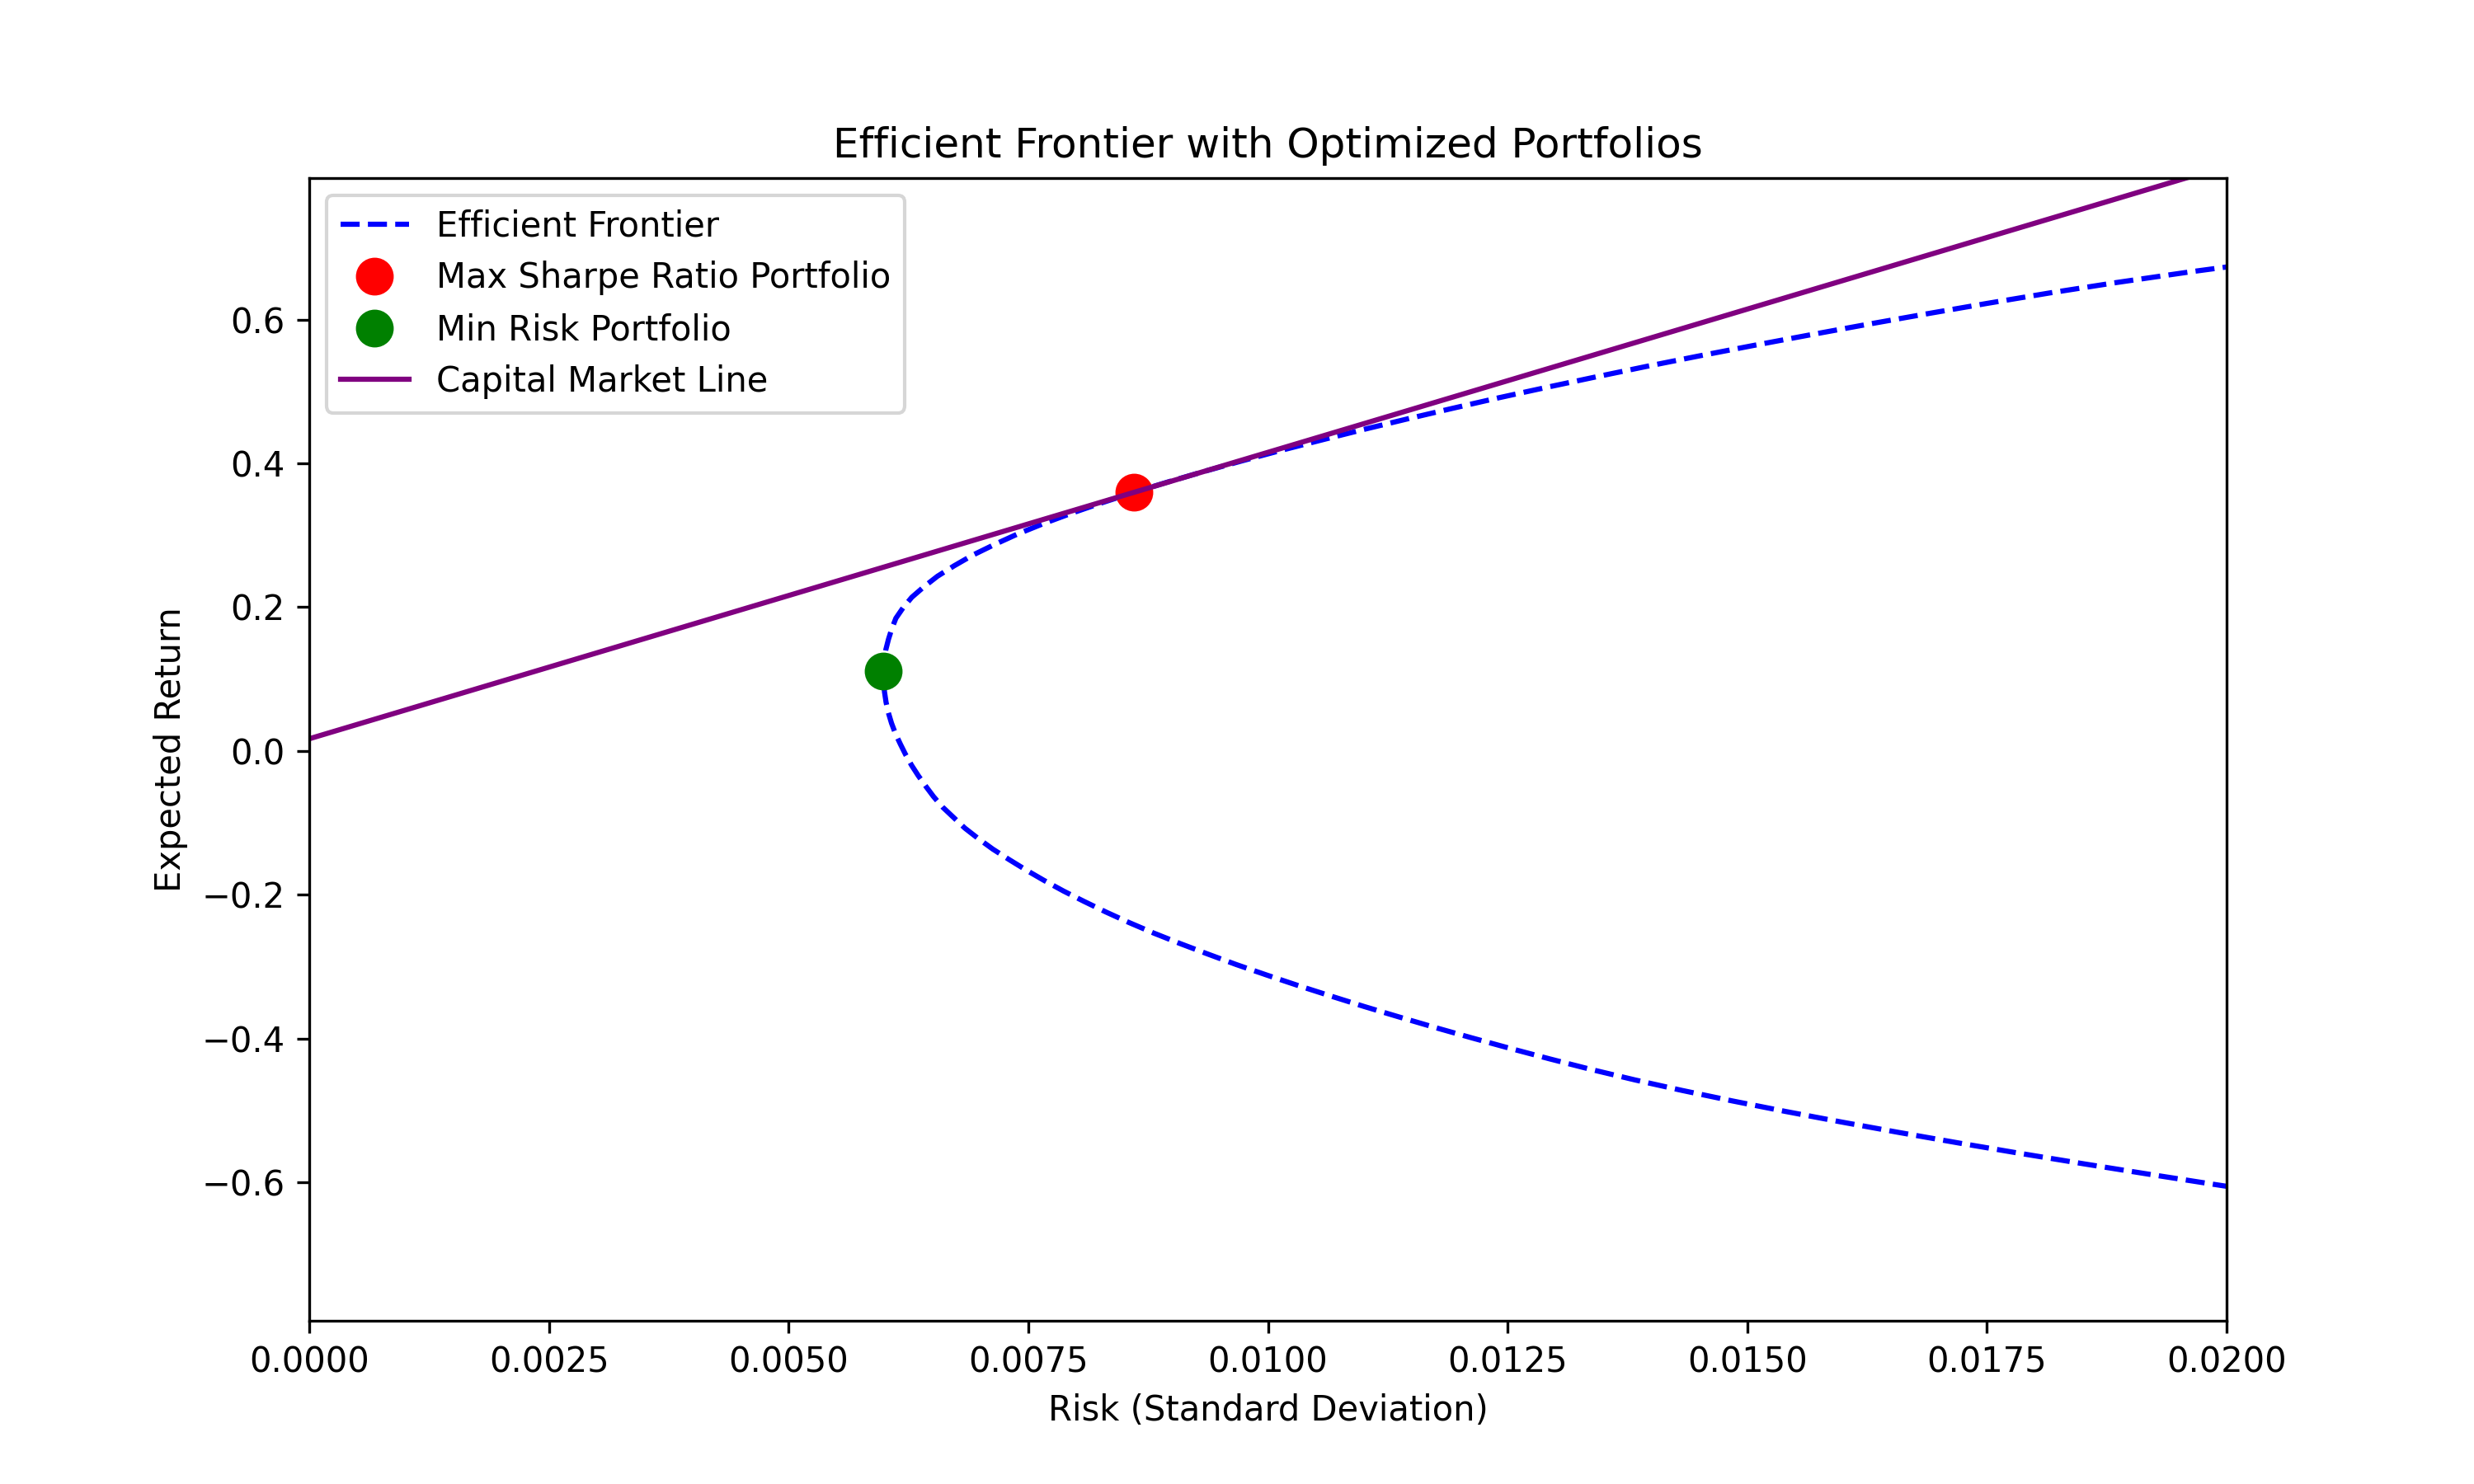
\includegraphics[width=0.8\textwidth]{figures/efficient_frontier.png}
    \caption{Plot showing the efficient frontier}
    \label{fig:efficient_frontier}
\end{figure}

\subsection{The Tangent Portfolio and The Capital Market Line}
% The tangent portfolio is the optimal risky portfolio, and it is the portfolio that has the highest Sharpe ratio.
% The capital market line is the line that connects the risk-free rate to the tangent portfolio.
% We now show the capital market line, and how to construct it.

The capital market line (CML) is the line that connects the risk-free rate to the tangent portfolio.
The tangent portfolio is the optimal risky portfolio, and it is the portfolio that has the highest Sharpe ratio.
The Sharpe ratio is given by:
\begin{equation}
    \label{eq:sharpe_ratio}
    S = \frac{E[R_p] - R_f}{\sigma_p}
\end{equation}
Where:
\begin{itemize}
    \item $S$ is the Sharpe ratio
    \item $E[R_p]$ is the expected return of the portfolio
    \item $R_f$ is the risk-free rate
    \item $\sigma_p$ is the standard deviation of the portfolio
\end{itemize}

The Sharpe ratio is a measure of the risk-adjusted return of a portfolio, and it is used to compare the performance of different portfolios.
The higher the Sharpe ratio, the better the portfolio's return per unit of risk.

Going back to Figure \ref{fig:efficient_frontier}, we can see that the CML is the line that connects the risk-free rate to the tangent portfolio.
It represents the set of all efficient portfolios that can be constructed by combining the risk-free asset with the tangent portfolio.
The line to the left of the tangent portfolio represents having a positive exposure to the risk-free asset, and the line to the right of the tangent portfolio represents having a negative exposure to the risk-free asset.
A negative exposure means taking out a loan to invest in the tangent portfolio.

The formula for the CML is given by some weight on the risk free rate, and some weight on the tangent portfolio:
\begin{equation}
    \label{eq:cml}
    E[R_p] = w_f R_f + w_t E[R_t]
\end{equation}
Where:
\begin{itemize}
    \item $E[R_p]$ is the expected return of the portfolio
    \item $w_f$ is the weight of the risk-free asset in the portfolio
    \item $R_f$ is the risk-free rate
    \item $w_t$ is the weight of the tangent portfolio in the portfolio
    \item $E[R_t]$ is the expected return of the tangent portfolio
\end{itemize}

